% !TeX root = ../libro.tex
% !TeX encoding = utf8

\setchapterpreamble[c][0.75\linewidth]{%
	\sffamily
	
    En esta sección se adentrará en el marco teórico del aprendizaje estadístico. No se abarcará esta teoría desde una perspectiva general en su totalidad, si no que se particularizará para el caso de aprendizaje supervisado, en particular, la clasificación y en algunas partes, para simplificar, se considerará el caso de clasificación binaria. El capítulo comenzará presentando los conceptos que conformarán el punto de partida y se definirá el concepto de aprendizaje. Tras lo cual se definirán los dos tipos de errores que se usarán en lo que sigue, el error empírico y el error de generalización. El primero está relacionado con los datos de la muestra y el segundo con lo que ocurre fuera de ella. Con esto, se fijará el paradigma de aprendizaje, que será el criterio de minimización del riesgo empírico (ERM).   Después se introducirá un marco teórico llamado PAC, que identificará la clase de funciones aprendibles que dan una solución aproximada en términos del número de elementos que se usen en la muestra. Dichas clases de funciones, a las cuales se las conoce como PAC aprendibles presentan algunas restricciones, entonces el objetivo siguiente será aplicar el concepto de aprendizaje por convergencia uniforme para poder relajar dichas restricciones y obtener un resultado más general sobre la clase de funciones que son PAC aprendibles.  Sin embargo, no se podrá abarcar todas las clases de funciones y para ello habrá que recurrir a otra teoría conocida como la dimensión de Vapnik Chervonenkis (dimensión VC). También se comentarán cotas de generalización las cuales son muy útiles e importantes en la teoría del aprendizaje y que se basan principalmente en la desigualdad de Hoeffding. Estas cotas son desigualdades probabilísticas que acotan la probabilidad de que el error empírico y el de generalización se alejan en más de un umbral. Después se presentará el teorema fundamental del aprendizaje estadísico que relaciona la dimensión VC con el la teoría PAC y con la convergencia uniforme anteriormente comentada.     Para terminar se comentará otro paradigma que usa un punto de vista distinto al de la teoría VC en cuanto a la generalización y aproximación el cual se basa en descomponer la esperanza del error de generalización en dos componentes, el sesgo y la varianza. \\
    
    
    La bibliografía en la que nos hemos apoyado para la elaboración de este capítulo ha sido, \cite{FML,Vapnik,data,M.Mitchell,UML}.    
    
    
	\par\bigskip
}
\chapter{Teoría del aprendizaje Estadístico}\label{ch:AprendizajeEstadistico}


    
    \newpage 
    \section{Introducción}
    
    Antes de todo, pongamos un pequeño ejemplo recogido de \cite{UML} el cual nos va a dar una idea intuitiva para entender mejor lo que sigue. Supongamos que hemos llegado a una pequeña isla donde las papayas son un ingrediente principal para la elaboración de las comidas. Sin embargo, no la hemos probado en nuestra vida y tenemos que aprender a predecir si una papaya que veas en el mercado está sabrosa o no. Primeramente necesitamos conocer en qué características fijarnos para predecir, por ejemplo, podemos usar el color; si es un verde muy oscuro, más claro, naranja, el tasto; si es muy suave, suave, rugosa o muy rugosa. Nuestro modo de aprender consiste en tener unas papayas de las cuales podamos saber si son sabrosas o no y fijarnos en que características tienen, para luego predecir que las sabrosas son aquellas con las características comunes a las papayas que nos gustaron y teníamos previamente. \\
    
    Vamos a tratar una serie de conceptos previos que nos ayudarán a ponernos en contexto para poder definir lo que es un problema de aprendizaje:
    
    \begin{itemize}

        \item Algoritmo de aprendizaje: Es un algoritmo, $\mathcal{A}$, al cual se le pasa una entrada, y genera una salida. El proceso interno que realiza $\mathcal{A}$ para proporcionar la salida se conoce como aprendizaje. Lo denotamos como $\mathcal{A}$.

        \item Elementos de Entrada:
                
                \begin{itemize}
                    \item Espacio Muestral: Es un población (conjunto) $\X$ que contiene a todas las posibles entradas, $x$, que son vectores de características. Estos elementos son los que pretendemos etiquetar y están generados de acuerdo a una distribución de probabilidad $P$\footnote{Cometiendo un abuso de notación, en este capítulo denotaremos a la distribución de probabilidad de una variable aleatoria $X$ como $P(X)$ (usando paréntesis) ó $P$. También notaremos como $\Pb$  cualquier medida de probabilidad definida sobre un espacio medible} desconocida pero fija a lo largo del tiempo. También los llamaremos \textit{instancias} o \textit{ejemplos}. 
                    \item Espacio de Etiquetas: Es un conjunto $\Y$ que contiene todas las posible etiquetas.
                    \item  Datos de entrenamiento: Es un conjunto finito $S \subset \X x \Y$. Estos son los elementos que se usarán para aprender, es decir, aquellos a los que $\mathcal{A}$ tendrá acceso. 
                \end{itemize}
          
                
        \item Elementos de Salida: El algoritmo de aprendizaje proporciona una salida, que será una aplicación $h:\X \to \Y$. Esta función se la conoce como \textit{predictor}, \textit{hipótesis} o \textit{clasificador} y será elegida dentro de un conjunto de posibles hipótesis denotado como $\mathcal{H}$. El clasificador será usado para etiquetar (predecir) nuevos ejemplos.
        
        \item Función objetivo-Distribucón Objetivo: La función objetivo es una aplicación (variable aleatoria) $f:\X \to \Y$ que a cada $x\in \X$ le hace corresponder una etiqueta $y \in \Y$. Es una función desconocida y es la que trataremos de aprender. De ella solo conocemos su imagen sobre $\X$. De este modo definimos el conjunto ${Z = \{ (x,f(x)): x \in \X\}}$ como el conjunto formado por los ejemplos con su respectiva etiqueta. En la práctica, las etiquetas no se generan de manera determinista, ya que existe ruido en el proceso, esto implica que la salida no está totalmente determinada por la entrada. Entonces en vez de $y = f(x)$, podemos considerar la salida $y$ como una variable aleatoria que está afectada por la entrada $x$. Más formalmente, estamos hablando de una distribución objetivo (distribución de probabilidad) $P(y|x)$ en vez de una función objetivo $y = f(x)$. Partiendo de una distribución objetivo, podemos considerar $P(y|x) = 0$ para todo $y\in Y$ excepto cuando $y=f(x)$, obteniendo así la función objetivo. 
        
        \item Generación de datos de entrenamiento: Se toma una muestra finita de $\X$ de manera independiente e idénticamente distribuida (i.i.d.) generada por una distribución conjunta $P(x,y) = P(x)P(y|x)$\footnote{Hay una diferencia entre el papel que juega $P(y|x)$ y $P(x)$. Aunque ambas modelen aspectos probabilísticos de $x$ e $y$. Tenemos que $P(y|x)$ modela qué es lo que se está intentando aprender, mientras que $P(x)$ cuantifica la importancia relativa del punto $x$ al ser elegido}. Podemos considerar la función objetivo o la distribución objetivo sin que haya pérdida de generalidad. La hipótesis $(i.i.d.)$ la denotaremos más adelante como $S\sim P^m$ donde $m$ es el tamaño de $S$ y $P^m$ denota la probabilidad inducida sobre la $m$-tupla al aplicar $P$ para escoger cada elemento de la tupla de manera independiente de los otros elementos. \\ 
        
      
        \item Medida de error: En el proceso de aprendizaje es muy común que se comentan errores, esto motiva la existencia de una aplicación que se use para cuantificar dicho error. Sea $\mathcal{H}$ un conjunto de hipótesis, sea $\mathcal{Z}$ un dominio, se define el error como una aplicación $P$-integrable $\ell: \mathcal{H} \times \mathcal{Z} \to \R^{+}$ que toma valores en los reales positivos. Para problemas de predicción consideramos $\mathcal{Z} = \X \times \Y$. Definimos la función de error de generalización como la esperanza del error de la hipótesis $h\in \mathcal{H}$ con respecto a la distribución de probabilidad $\Pc$ sobre $\mathcal{Z}$,
        \begin{equation}\label{eq:general_loss_function}
            R_{P}(h) := \E_{z\sim P} [\ell(h,z)] = \int_{\mathcal{Z}} \ell(h,z) dP(z)
        \end{equation}
    \end{itemize}
    
    En las definiciones anteriores partimos de un espacio probabilístico $(\Omega,\mathcal{F},\Pb)$, donde generalmente $\Omega = \R^n$, $\mathcal{F} = \mathcal{B}(\R^n)$ y  $\Pb$ cualquier medida de probabilidad. La distribución de probabilidad $P$ asumimos que es de cualquier variable aleatoria $X:(\Omega, \mathcal{F})) \to (\mathcal{Z}, \mathcal{B}(\mathcal{Z}))$, donde $\mathcal{B}(\mathcal{Z})$ es el $\sigma$-álgebra de Borel generado por $\mathcal{Z}$, por lo que la distribución $P = \Pb \circ X^{-1}$ tiene como dominio $(\mathcal{Z}, \mathcal{B}(\mathcal{Z}))$. De manera similar, el error $\ell(h,\cdot)$ definido en $(\mathcal{Z}, \mathcal{B}(\mathcal{Z}))$ y con valores en $(\R^+,\mathcal{B}(\R^+))$ es una variable aleatoria para todo $h \in \mathcal{H}$, y la función de error es la esperanza de dicha variable aleatoria. \\
    

    Con estos conceptos claros, estamos en condiciones de formalizar la definición de aprendizaje. Según Mitchell  (\cite{M.Mitchell}) \textit{Un programa aprende de la experiencia E, con respecto a alguna clase de tarea T y medida de rendimiento M, si el rendimiento del algoritmo para cumplir la tarea T mejora con respecto a M gracias a la experiencia E.} En esta definición entendemos tarea como cualquier objetivo que pretendemos que nuestro algoritmo aprenda, algunos ejemplos de tarea son clasificación y regresión. Entendemos la experiencia $E$ como un conocimiento del cual disponemos. La medida $M$ es la responsable de evaluar las habilidades del algoritmo. \\
    
    Este formalismo dado por Mitchell, es bastante más general del que nos atañe, en nuestro caso, podemos particularizarlo a clasificación mediante aprendizaje supervisado y decir que el problema de aprendizaje se basa en que partiendo de una población $\X$ cuyos elementos son generados por una distribución $P$ la cual desconocemos, $\Y$ el conjunto de las etiquetas, y una distribución objetivo $P(y|x)$. Tomar un conjunto de entrenamiento $S=\{(x_i,y_i) : i = \{1,...,n\}\}$ donde las instancias son generadas por la distribución conjunta $P(x,y) = P(x)P(y|x)$ y extraídas de manera $i.i.d.$ de $\X \times \Y$. Introducir dicho conjunto de entrenamiento en el algoritmo $\mathcal{A}$ y generar una hipótesis $g \in \mathcal{H}$ tal que minimice la función de error empleada para que de este modo $g \approx P(y|x)$. Lo anterior lo podemos resumir de manera visual en la imagen \ref{fig:EsquemaAASupervisado}
    
    \begin{figure}[htpb]
        \centering
        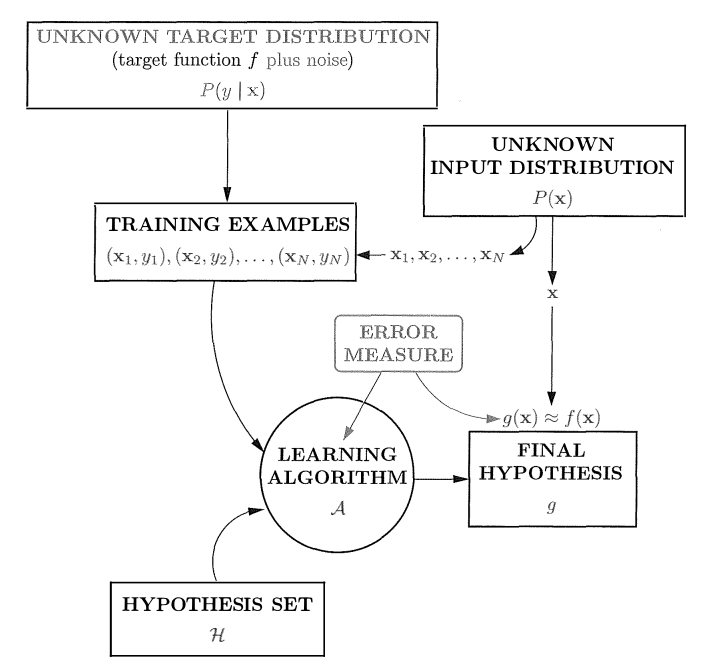
\includegraphics[scale=0.6]{img/Esquema AASupervisado.png}
        \caption{Esquema del problema de Aprendizaje Supervisado. Imagen extraída de \cite{data}}
        \label{fig:EsquemaAASupervisado}
    \end{figure}
    
%%%%%%%%%%%%%%%%%%%%%%%%%%%%%%%%%%%%%%%%%%%%%%%%%%%%%%%%%%%%%%%%%%%%%
%%%%%%%%%%%%%%%%%%%%%%%%%%%%%%%%%%%%%%%%%%%%%%%%%%%%%%%%%%%%%%%%%%%%%
%%%%%%%%%%%%%%%%%%%%%%%%%%%%%%%%%%%%%%%%%%%%%%%%%%%%%%%%%%%%%%%%%%%%%

\section{Paradigma ERM}


    
        
        Como se mencionó anteriormente, $\A$ recibe como entrada un conjunto de entrenamiento $S$, muestreado de manera $i.i.d.$ de $Z$ y debe proporcionar un predictor $h_S:\X \to \Y$. El objetivo es encontrar dicha hipótesis $h_S$ que minimice el error respecto de la distribución $P$ y $P(y|x)$. Tanto $P$ como $P(y|x)$ son desconocidas, el algoritmo no va a tener acceso al error de generalización (también conocido como error fuera de la muestra o error verdadero) definido en \eqref{eq:general_loss_function}, esto motiva la siguiente definición, la cual se conoce como error de entrenamiento, error empírico o error dentro de la muestra.
    
        
            \begin{definicion}[Error empírico - clasificación binaria]
                Dada $h\in \mathcal{H}$, $\ell$ una función de error y  ${S=\{(x_1,y_1),...,(x_m,y_m)\}}$ un conjunto de entrenamiento, se define el error empírico como 
                \begin{equation}
                \Rh_{S}(h) := \frac{1}{m} \sum_{i=1}^m [\mathbb{1}_{h(x_i) \not= y_i}]
                \end{equation}
                \noindent Cuando no haya lugar a dudas sobre el conjunto de entrenamiento, notaremos $\hat{R}(h)$ en vez de $\hat{R}_S(h)$
            \end{definicion}
            
            
        \begin{proposicion}\label{prop:esperanza del error empirico}
            Dada $h \in \mathcal{H}$ y un  conjunto de entrenamiento S extraído de manera $i.i.d$, entonces
            
            \begin{equation}
                \E[\hat{R}(h)] = R(h)
            \end{equation}
            \end{proposicion}
            
            \begin{proof}
            Usando la linealidad de la esperanza y la hipótesis, tenemos que 
            \begin{equation}
                \begin{aligned}
                    \E_{S \sim P^m} [\hat{R}(h)] & = \frac{1}{m}\sum_{i=1}^m \E_{S \sim P^m}[1_{h(x_i)\neq y_i}]  \\
                     & = \E_{x \sim P}[1_{h(x)\neq y}]  \\
                     & = R(h)
                \end{aligned}
            \end{equation}
            \end{proof}
        
        El error de generalización, desgraciadamente no vamos a poder calcularlo. Pero gracias al conjunto de entrenamiento tenemos una representación del mundo exterior disponible para ser usada por el algoritmo. Además, gracias a la proposición anterior, tenemos que bajo ciertos supuestos, la esperanza del error empírico es el error de generalización. Nuestros objetivo ahora es conseguir cumplir: 
        
        \begin{equation}\label{eq:objetivos_aprendizaje}
            \begin{aligned}
                \hat{R}(h) \approx 0 ,&&    \hat{R}(h) \approx R(h)
            \end{aligned}
        \end{equation}
        
        \noindent De este modo, al ser muy pequeño el error empírico y al estar muy próximo al error de generalización, vamos a lograr que el erro de generalización esté también próximo a cero, que sería lo ideal. \\
        
        
        El primer objetivo lo logramos buscando una hipótesis que minimice el error empírico, a este paradigma se le conoce como ERM, del inglés, \textit{Empirical Risk Minimization}. Más formalmente se busca una hipótesis $h_S \in \mathcal{H}$ tal que 
        \begin{equation}
           h_S \in argmin_{h \in \mathcal{H}} \hat{R}_S(h)
        \end{equation}
        donde $argmin$ denota el conjunto de hipótesis de $\mathcal{H}$ para las que se alcanza un mínimo sobre $\hat{R}_S(h)$ \\
        
        Con este paradigma vamos a tener que hacer frente a un gran inconveniente, que es la aparición de sobreaprendizaje, del cual hablaremos más adelante. Solo diremos que el sobreaprendizaje ocurre cuando encontramos una hipótesis $h^* \in \mathcal{H}$ de tal manera que $\Hat{R}(h^*)$ sea un valor muy pequeño y $R(h^*)$ un valor muy grande, es decir, $\hat{R}(h^*) \not\approx R(h^*)$, faltando de este modo al cumplimiento del primer objetivo en \eqref{eq:objetivos_aprendizaje} \\
        
        Para lidiar con esto, se puede restringuir la clase de hipótesis, lo que sesga hacia un conjunto particular de clasificadores. Este método es lo que se conoce como \textit{sesgo inductivo}, con esto se logra cumplir el segundo objetivo ($\Rh \approx R$) en detrimento del primero ($\Rh \approx 0$), ya que al restringir la clase de hipótesis puede ocurrir que no incluyamos las hipótesis para las que se alcance un mínimo. \\
        
        
        
        Con motivo de simplificar las cosas, particularizaremos al caso de clasificación binaria, es decir, cuando $\Y = \{0,1\}$. También se considerará el concepto de función objetivo, $f$, en vez de distribución objetivo, $P(y|x)$, aunque en verdad se puede considerar cualquiera. Vamos a definir los errores para este caso,

    
            \begin{definicion}[Error 0-1]
            Dado $h \in \mathcal{H}$, una función objetivo $f$, se define el error $0-1$ para todo ${z = (x,f(x))}$ como
            \begin{equation}
                \ell_{0-1}(h,z) = 
                \left\{
                \begin{array}{cc}
                     0 & h(x) = y \\
                     1 & h(x) \neq y
                \end{array}
                \right.
             \end{equation}
            \end{definicion}
        
        
            \begin{definicion}[Error de Generalización, Clasificación Binaria]\label{def:errorGeneralizacion}
            Dada una hipótesis $h \in \mathcal{H}$, una función objetivo $f$ y una distribución de probabilidad subyacente $P$ definimos el error de generalización de $h$ como
            \begin{equation}
                R_{P,f}(h) := \Pb_{x \sim P}[h(x) \neq f(x)] = P(\{x: h(x) \neq f(x)\}) \quad \forall x \in \X
            \end{equation}
            \noindent Los subíndices $P,f$ hacen énfasis en la distribución subyacente y en la función objetivo, pero cuando no quepa lugar a duda lo notaremos como $R(h)$ omitiendo los subíndices. \\
            \end{definicion}
        
\section{Aprendizaje PAC}

    A la hora de diseñar y analizar algoritmos que aprenden de los ejemplos se pueden plantear una serie de cuestiones tales como ¿Cuántos ejemplos son necesarios para aprender con éxito? ¿Existe un modelo general de aprendizaje? En esta sección vamos a formalizar y a tratar estas cuestiones introduciendo el marco de aprendizaje correcto probablemente aproximado (PAC). Dicho marco nos ayudará a definir la clase de funciones aprendibles en términos del número de puntos de la muestra necesarios para lograr una solución aproximada. \\
    
    Vamos a especificar cuándo una clase de hipótesis es PAC aprendible, para ello vamos a considerar una función objetivo $f$, en vez de una distribución objetivo $P(x,y)$, también consideraremos el caso de clasificación binaria aunque al final generalizaremos para cualquier función de pérdida. Vamos a suponer también lo que se conoce como hipótesis o asunción de realizabilidad. \\
    
    
    \begin{definicion}[Asunción de realizabilidad]
    La hipótesis o asunción de realizabilidad se basa en suponer que existe $h^* \in \mathcal{H}$ tal que $R_{P,f}(h^*) = 0$. 
    \end{definicion}
    
    \begin{observacion}
    Notamos que esta asunción implica con probabilidad 1 sobre una muestra aleatoria, $S$, donde las instancias son muestreadas acorde a $P$ y etiquetadas por $f$, que para cada hipótesis $h_S \in \Hc$ elegida acorde al criterio ERM, $\hat{R}_S(h_S) = 0$. Por lo que en este caso estamos más interesados en el error de generación que en el error empírico. \\
    \end{observacion}
    
    Como $R_{P,f}(h_S)$ depende del conjunto de entrenamiento y este se elige de manera aleatoria, tenemos una aleatoriedad implícita en la elección de $h_S$ y en consecuencia, en el error $R_{P,f}(h_S)$. No es cierto pensar que el conjunto $S$ baste para guiar la elección del algoritmo a una buena hipótesis ya que siempre existe una probabilidad de que los datos de entrenamiento que se han extraído sean muy pocos representativos de la distribución $P$. De aquí en adelante denotaremos a la probabilidad de elegir una muestra no representativa por $\delta$ y llamaremos $(1-\delta)$ el \textit{parámetro de confianza} de nuestra predicción. Además, como no podemos garantizar una predicción perfecta de las etiquetas, introducimos otro parámetro para la calidad de la predicción y lo llamaremos \textit{parámetro de precisión} denotado como $\epsilon$. Interpretaremos $R_{P,f}(h_S) > \e$ de manera negativa, viéndolo como un fallo o fracaso en elección de la hipótesis, por rebasar el umbral de precisión (en la proposición \ref{pro:cp_negativo} daremos una cota superior para la probabilidad de que ocurra este suceso), mientras que $R_{P,f}(h_S) \leq \e$ lo veremos como una predicción aproximadamente correcta. \\
    
    
    
        \begin{definicion}[Aprendizaje PAC]
        Una clase de hipótesis $\mathcal{H}$ es PAC aprendible cuando exista una función $m_{\mathcal{H}}:(0,1)^2 \to \N$ y un algoritmo de aprendizaje $\mathcal{A}$ con la siguiente propiedad: Para todo $\e, \delta \in (0,1)$, para cada distribución $P$ sobre $\X$ y para cada función objetivo $f:\X \to \{0,1\}$, si se cumple la hipótesis de realizabilidad con respecto $\Hc, P,f$, entonces cuando ejecutamos el algoritmo de aprendizaje $\A$ en $m\geq m_{\Hc}(\e,\de)$ $i.i.d.$ ejemplos generados por $P$ y etiquetados por $f$, $\A$ devuelve una hipótesis $h \in \Hc$ tal que,
            \begin{equation}
                \Pb_{S\sim P^m}[R_{P,f}(h) \leq \e] \geq 1 - \de
            \end{equation}
            
        \end{definicion}
        
    En esta definición, la \textit{precisión}, $\e$, determina como de lejos está el clasificador del óptimo y corresponde a la parte \textit{AC} de \textit{PAC}, del inglés, \textit{approximately correct}. El parámetro de confianza, $(1-\de)$ indica cómo de probable es que el clasificador cumpla ese requisito la precisión, y corresponde a la parte de \textit{probability} del \textit{PAC}. \\
    
    La función $m_{\mathcal{H}}:(0,1)^2 \to \N$ determina la complejidad de la muestra para aprender $\Hc$, esto es, cuantos ejemplos se requieren para garantizar una solución PAC. La complejidad de la muestra depende e la precisión ($\e$) y de la confianza ($\de$), pero también depende de algunas propiedades de la clase de hipótesis $\Hc$ que veremos más adelante. \\
    


    \begin{proposicion}\label{pro:cp_negativo}
        Sea $f$ una función de etiquetado, $S_{|x} = \{(x_1,...,x_m\}$ un conjunto de entrenamiento y $P$ una distribución de probabilidad subyacente sobre la que se han extraído las muestras de manera $(i.i.d.)$. Suponemos también que el conjunto de hipótesis $\mathcal{H}$ es finito y que se cumple la hipótesis de realizabilidad, entonces
        
        \begin{equation}
            P^m(\{S_{|x} : R_{P,f}(h_S) > \e\}) \leq |\mathcal{H}| e^{-\e m}
        \end{equation}
    \end{proposicion}
    
    \begin{proof}
     Consideramos el conjunto de hipótesis incorrectas
         
         \begin{equation}
             \Hc_B = \{ h \in \Hc : R_{P,f} > \e\}
         \end{equation}
    
    \noindent y el conjunto de de las muestras de entrenamiento para las que existe un hipótesis incorrecta que hacen al error empírico cero. 
    
        \begin{equation}
            M = \{ S_{|x} : \exists h \in \Hc_B , \hat{R}_S(h) = 0 \}
        \end{equation}
 
    Podemos ver el conjunto $M$ como aquel en el que las hipótesis parecen buenas sin serlo. El objetivo es acotar la probabilidad del suceso $R_{P,f}(h_S) > \e$. Por la hipótesis de realizabilidad se sigue que el suceso $R_{P,f}(h_S) > \e$ ocurre solo si existe $h\in \Hc_B$ con $\hat{R}_S(h) = 0$, por lo que
    \begin{equation}
        \{S_{|x}: R_{P,f}(h_S) > \e \} \subseteq M
    \end{equation}
    
    \noindent Reescribiendo M como $M = \bigcup_{h \in \Hc_B}\{ S_{|x}: \hat{R}_S(h) = 0\}$, tenemos que     
    \begin{equation}
        \begin{aligned}
            P^m(\{ S_{|x}:R_{P,f}(h_S) > \e \}) & \leq  P^m\Big(\bigcup_{h \in \Hc_B} \{ S_{|x}:\hat{R}_S(h) = 0 \} \Big) \\
            & \leq \sum_{h \in \Hc_B} P^m(\{ S_{|x}:\hat{R}_S(h) = 0 \} ) \\
            & = \sum_{h \in \Hc_B} P^m(\{ S_{|x}: h(x_i) = f(x_i) \; \forall i \} ) \\
            & = |\Hc_B| (1 - R_{P,f}(h))^m  \\
            & \leq  |\Hc| (1 - \e)^m  \\
        \end{aligned}
    \end{equation}

    \noindent Usando que $1 - e \leq e^{-\e}$ se sigue que $|\Hc| (1 - \e)^m  \leq |\Hc|e^{-m \e}$
    
    \end{proof}

    
    \begin{corolario}
    Bajo la asunción de realizabilidad, toda clase de hipótesis finita es PAC aprendible verificando, 
    
    \begin{equation}
        m_{\Hc} (\e, \de) \leq \lceil \frac{log(|\Hc|/\de)}{\e} \rceil
    \end{equation}
    
    \end{corolario}
    
    \begin{observacion}
    Notamos que el error de generalización se aproxima a cero cuando el tamaño del conjunto de entrenamiento aumenta.
    \end{observacion}
    
    
    
    
%%%%%%%%%%%%%%%%%%%%%%%%%%%%%%%%%%%%%%%%%%%%%%%%%%%%%%%%%%%%%%%%%%%%%
%%%%%%%%%%%%%%%%%%%%%%%%%%%%%%%%%%%%%%%%%%%%%%%%%%%%%%%%%%%%%%%%%%%%%
%%%%%%%%%%%%%%%%%%%%%%%%%%%%%%%%%%%%%%%%%%%%%%%%%%%%%%%%%%%%%%%%%%%%%    
    
    
    \subsection{Agnostic PAC}
        La definición de PAC que hemos dado no es para nada general, ya que parte de la premisa de realizabilidad, que es una hipótesis bastante fuerte la cual no se cumple en la mayoría de los casos. Motivo por el cual vamos a generalizarla para abarcar un mayor número de casos. Para ello relajamos las hipótesis eliminando la asunción de realizabilidad y suponiendo una distribución objetivo conjunta $P(x,y)$ en vez de una función objetivo, $f$.\\
    
        \begin{definicion}[Agnostic-PAC]
         Una clase de hipótesis $\Hc$ es PAC agnóstica aprendible si existe una función $m_{\Hc}:(0,1)^2 \to \N$ y un algoritmo de aprendizaje $\A$ con la siguiente propiedad: Para todo $\e, \de \in (0,1)$ y para todo distribución $P$ conjunta sobre $\X \times 
         \{0,1\}$, cuando ejecutemos el algoritmo de aprendizaje sobre $m \geq m_{H}$ ejemplos $i.i.d.$ generados por la distribución conjunta $P$, el algoritmo devuelve una hipótesis $h \in \Hc$ tal que 
         
         \begin{equation}
             \Pb_{S \sim P^m}[R_P(h) - min_{h' \in \Hc}R_P(h') \leq \e] \geq 1 - \de
         \end{equation}
                
         \end{definicion}
                
        
        Rizando aún más el rizo en pos de lograr una mayor generalización, notamos que la definición anterior solo abarca el caso de clasificación binaria, es decir, los supuestos en los cuales $\Y = \{0,1\}$ y $\ell = \ell_{0-1}$ y la función de error de generalización viene dada por \ref{def:errorGeneralizacion}. 
        
        \begin{definicion}[Agnostic-PAC  para una función de pérdida general]
        Una clase de hipótesis $\Hc$ es PAC-Agnóstica con respecto a un conjunto $Z \subset \X \times \Y$ y una función de pérdida medible $\ell: \Hc \times Z \to \R^+$ cuando exista una función $m_{\Hc}:(0,1)^2 \to \N$ y un algoritmo de aprendizaje $\A$ cumpliendo la siguiente propiedad: Para cada $\e ,\de \in (0,1)$ y para cada distribución $P$ sobre $Z$, cuando ejecutamos el algoritmo de aprendizaje sobre  $m \geq m_{\Hc}(\e, \de)$ ejemplos $i.i.d.$ generados por $P$, el algoritmo devuelve $h \in \Hc$ tal que,
        
        \begin{equation}
            \Pb_{S\sim P}[L_P(h) - min_{h' \in \Hc} L_P(h') \leq \e] \geq 1 - \de
        \end{equation}
        
        donde $L_D(h) = \E_{z\sim P}[\ell(h,z)]$ 
        
        \end{definicion}
    


%%%%%%%%%%%%%%%%%%%%%%%%%%%%%%%%%%%%%%%%%%%%%%%%%%%%%%%%%%%%%%%%%%%%%
%%%%%%%%%%%%%%%%%%%%%%%%%%%%%%%%%%%%%%%%%%%%%%%%%%%%%%%%%%%%%%%%%%%%%
%%%%%%%%%%%%%%%%%%%%%%%%%%%%%%%%%%%%%%%%%%%%%%%%%%%%%%%%%%%%%%%%%%%%%
\subsection{Aprendizaje por Convergencia Uniforme}

    En la sección anterior, vimos que una clase de hipótesis finita es PAC aprendible suponiendo la hipótesis de realizabilidad. En esta sección vamos eliminar dicha asunción para demostrar que cualquier clase de hipótesis finita es Agnostic-PAC aprendible. Para ello vamos a aplicar el concepto de convergencia uniforme en el sentido de que vamos a necesitar que uniformemente sobre todas las hipótesis de la clase de hipótesis, el riesgo empírico esté próximo al riesgo verdadero. \\
    
    
    \begin{definicion}[muestra $\e$-representativa]
    Se dice que un conjunto de entrenamiento es $\e$-representativo con respecto a un dominio $Z$, una clase de hipótesis $\Hc$, una función de pérdida $\ell$ y una distribución subyacente $P$ cuando,
    \begin{equation}
        |\hat{R}_{S}(h) - R_{P,f}(h)| \leq \e \quad \forall h \in \Hc
    \end{equation}
    \end{definicion}

    
    \begin{lema}\label{lema:UC}
    Sea $S$ un conjunto de entrenamiento $\frac{\e}{2}$-representativo con respecto a $Z, \Hc, \ell$ y $P$. Entonces, cualquier hipótesis $h_S \in argmin_{h \in \Hc}L_S(h)$ satisface que,
    \begin{equation}
        R_{P,f}(h_S) \leq min_{h \in \Hc} R_{P,f}(h) + \e
    \end{equation}
    \end{lema}
    
    El lema anterior viene a decir que para cualquier muestra que sea $\e/2$-representativa el criterio ERM garantiza una buena hipótesis de salida. La demostración es prácticamente inmediata, para ello basta considerar $h\in \Hc$ arbitraria, entonces
    
    \begin{equation}
        R_{D,f}(h_S) \leq \Rh_S(h_S) + \frac{\e}{2} \leq \Rh_S(h) + \frac{\e}{2} \leq R_{P,f}(h) + \frac{\e}{2} + \frac{\e}{2} = R_{P,f}(h) + \e
    \end{equation}
    
    \noindent al ser $h$ una hipótesis arbitraria, tenemos que lo anterior se cumple para todo $h \in \Hc$. 
    
    
    
    
    \begin{definicion}[Convergencia uniforme]\label{def:UC}
       Decimos que una clase de hipótesis $\Hc$ cumple la propiedad de la convergencia uniforme (con respecto a un dominio $Z$ y una función de error $\ell$) cuando exista una función $m_{\Hc}^{UC}:(0,1)^2 \to \N$ tal que para cada $\e, \de \in (0,1)$ y para cada distribución de probabilidad, $P$, sobre $Z$, si el conjunto de entrenamiento, $S$, tiene $m\geq m_{\Hc}^{UC}(\e,\de)$ ejemplos tomados de manra $(i.i.d.)$ de acuerdo a $P$, entonces con probabilidad al menos $1-\de$ el conjunto de entrenamiento $S$ es $\e$-representativo.
    \end{definicion}
    
    Análogo a la definición de PAC, la función $m_{\Hc}^{UC}$ mide la complejidad de la muestra mínima, esto es, el número mínimo de ejemplos que necesitamos para asegurar con probabilidad al menos $1 - \de$ que la muestra es $\e$-representativa. El término \textit{uniforme} hace referencia a tener un tamaño de muestra fijo que funcione para todas las hipótesis de $\Hc$ y sobre todas las posibles distribuciones de probabilidad sobre el dominio. Aplicando el lema \ref{lema:UC} y la definición \ref{def:UC} obtenemos el siguiente corolario. \\
    
    \begin{corolario}\label{corolario:APAC-UC}
       Si una clase de hipótesis cumple la propiedad de convergencia uniforme. La clase de funciones es Agnostic-PAC aprendible con una complejidad de la muestra ${m_{H}(\e,\de) \leq m_{\Hc}^{UC}(\frac{\e}{2},\de)}$. Además, el paradigma $ERM_{\Hc}$ es un criterio de aprendizaje exitoso para $\Hc$. 
    \end{corolario}
   
   
   \begin{observacion}
   En vista del colorario anterior, la afirmación de que toda clase de hipótesis finita es Agnostic-PAC aprendible se producirá una vez se estableza que la convergencia uniforme se mantiene para clases de hipótesis finita. \\
   \end{observacion}
   
   
   \begin{proposicion}
   Sea $\Hc$ un conjunto de hipótesis finito, sea $Z$ un dominio y sea ${\ell:\Hc \times Z \to [0,1]}$ una función de error. Entonces, $\Hc$ cumple la propiedad de convergencia uniforme con una complejidad de la muestra,
   \begin{equation}
       m_{\Hc}^{UC}(\e,\de) \leq \lceil \frac{\log(2|\Hc|/\de)}{2\e^2} \rceil
   \end{equation}
   
   Además, $\Hc$ es Agnostic-PAC aprendible aplicando el criterio ERM y la complejidad de la muestra verifica,
   \begin{equation}
        m_{\Hc}(\e,\de) \leq  m_{\Hc}^{UC}(\e,\de) \leq \lceil \frac{\log(2|\Hc|/\de)}{2\e^2} \rceil
   \end{equation}
   \end{proposicion}

    \begin{proof}
    
    Fijamos $\e,\de$ y debemos encontrar un tamaño ,$m$, para una muestra, $S = (z_1,...,z_m)$, extraída de manera $i.i.d.$ de $P$ que verifique, con probabilidad al menos $1-\de$ que para todo $h \in \Hc$, $|\Rh_S(h) - R_{P}(h) | \leq \e$. Esto es,
        \begin{equation}
            P^m(\{ S: \forall h \in \Hc, | \Rh_S(h) - R_P(h) | \leq  \e \}) \geq 1 - \de
        \end{equation}
    \noindent y probar lo anterior equivale a probar que,
        \begin{equation}
            P^m(\{ S: \exists h \in \Hc, |\Rh_S(h) - R_P(h) | >  \e \}) \geq \de
        \end{equation}
    
    \noindent Escribiendo, 
        \begin{equation}
           \{ S: \exists h \in \Hc, |\Rh_S(h) - R_P(h) | >  \e \}) = \bigcup_{h\in\Hc} \{S: |\Rh_S(h) - R_P(h) | >  \e\}
        \end{equation}
        
    \noindent tenemos que,
        \begin{equation}\label{eq:aux01}
            P^m(\{ S: \exists h \in \Hc, |\Rh_S(h) - R_P(h) | >  \e \}) \leq \sum_{h \in \Hc} P^m(\{S: |\Rh_S(h) - R_P(h) | >  \e\})
        \end{equation}
    
    Recordemos que la definición general de los errores era, $R_P(h) = \E_{z\sim P}[\ell(h,z)]$ y $\Rh(h) = \frac{1}{m} \sum_{i=1}^m \ell(h,z_i)$. Como cada $z_i$ es muestreado de manera $i.i.d.$ de P, el valor esperado de la variable aleatoria $\ell(h,z_i)$ es $R_P(h)$. Además por la proposición \ref{prop:esperanza del error empirico} se sigue que $|R_{D}(h) - \Rh_S(h)|$ es la desviación de la variable aleatoria $\Rh_S(h)$ con respecto a su esperanza. Por lo que debemos de demostrar que los valores de $\Rh_S(h)$ se concentran en torno a su valor esperado. \\
    
    Fijamos $h \in \Hc$ y consideramos las variables aleatorias $\ell_i = \ell(h,z_i)$ para todo $i=1,...,m$. Como $(z_1,...,z_m)$ es una muestra de variables aleatorias $i.i.d.$, se sigue que $(\ell_1,...,\ell_m)$ también lo es. Vamos a asumir que el rango de $\ell(h,z_i) \in [0,1]$ para todo $i=\{1,...,m\}$. Denotamos $R_P(h) = \mu$ y aplicando la \textit{desigualdad de Hoeffding} \eqref{eq:Hoeffding} llegamos a que,
    
        \begin{equation} \label{eq:Hoeffding_error}
            P^m(\{S: |\Rh_S(h) - R_D(h)| > \e\}) = \Pb \Big[ \Big| \frac{1}{m} \sum_{i=1}^m \ell_i - \mu \Big| > \e \Big] \leq 2 \exp{(-2m\e^2)}
        \end{equation}
    \noindent y aplicando \eqref{eq:aux01} se sigue que,
        \begin{equation}
            P^m(\{ S: \exists h \in \Hc, |\Rh_S(h) - R_D(h)| > \e \}) \leq \sum_{h\in \Hc} 2 e^{-2m\e^2} = 2 |\Hc| e^{-2m\e^2}
        \end{equation}
    \noindent Eligiendo ahora,
        \begin{equation}
            m \geq \frac{\log(2 |\Hc|/\de)}{2\e^2}
        \end{equation}
    \noindent conseguimos
        \begin{equation}
             P^m(\{ S: \exists h \in \Hc, |\Rh_S(h) - R_P(h) | >  \e \}) \geq \de
        \end{equation}
        
        
    \noindent La segunda parte es inmediata del corolario \ref{corolario:APAC-UC}
    \end{proof}


%%%%%%%%%%%%%%%%%%%%%%%%%%%%%%%%%%%%%%%%%%%%%%%%%%%%%%%%%%%%%%%%%%%%%
%%%%%%%%%%%%%%%%%%%%%%%%%%%%%%%%%%%%%%%%%%%%%%%%%%%%%%%%%%%%%%%%%%%%%
%%%%%%%%%%%%%%%%%%%%%%%%%%%%%%%%%%%%%%%%%%%%%%%%%%%%%%%%%%%%%%%%%%%%%

\subsection{Cotas de Generalización para clases de hipótesis finitas}

Anteriormente se comentó que uno de los objetivos a los que aspiramos es a conseguir una hipótesis $g\in \Hc$ que se aproxime todo lo posible a la función o distribución objetivo. Para ello usamos una muestra $S$ extraída de manera $i.i.d.$ de acuerdo $P$ e intentamos minimizar el funcional $\Rh_S$. Sin embargo, puede ocurrir que $\Rh(g) \approx 0$ pero $\Rh_S \not\approx R_P$, lo cual indica que la hipótesis elegida no generaliza bien. Vamos a medir el grado de generalización dada una hipótesis $g \in \Hc$ como $|\Rh_S(g) - R_P(g)|$ y en esta sección daremos una serie de cotas de generalización. \\
    
    
    La desigualdad de Hoeffding nos da una manera de acotar el error de generalización en términos probabilísticos,
    
    \begin{equation}
        \Pb \Big[ \Big| \Rh_S(g) - R_{P}(g) \Big| \geq \e \Big] \leq 2 e^{-2m\e^2 }
    \end{equation}
    
    \noindent para cualquier $\e > 0$. Lo cual es equivalente a decir que con probabilidad al menos $1 - 2 e^{-2m\e^2 }$, ocurre que $|R_{P}(g) - \Rh_S(g)| \leq \e$, lo que implica que $R_{P}(g) \leq \Rh_S(g) + \e$, e identificando $\de = 2e^{-2m\e^2}$ y despejando $\e$ llegamos a que con probabilidad al menos $1 - \de$,
    
    \begin{equation}\label{eq:Generalization Bound}
        R_{P}(g) \leq \Rh_S(g) + \sqrt{\frac{1}{2m} \log{\frac{2}{\de}}}
    \end{equation}
    
    \noindent a esta desigualdad la llamamos cota de generalización porque acota $R_{P}$ en términos de $\Rh_S$. Por otro lado, la desigualdad  $|R_{P}(g) - \Rh_S(g)| \leq \e$, implica también que $R_{P}(g) \geq \Rh_S(g) - \e$. Esto importante tenerlo en cuenta, pero de manera más sutil. No solo queremos que la hipótesis $g$ que escojamos (la que minimize el error empírico) siga funcionando bien fuera de la muestra, sino que también queremos asegurarnos de que lo hicimos lo mejor que pudimos con la elección de la hipótesis en $\Hc$. La cota $R_{P}(g) \geq \Rh_S(g) - \e$, nos asegura que no podríamos hacerlo mejor, ya que para cada hipótesis $h$ con mayor riesgo empírico que $g$, $\Rh_S(g) \leq \Rh_S(h)$, tendremos $R_P(g) \geq R_P(h)$. \\
    
    Enunciemos lo anteriormente comentado,
    
    \begin{proposicion}
     Sea $\e >0$ fijo, y sea $S$ una muestra $i.i.d.$ de tamaño $m$. Entonces, para cualquier hipótesis $g:\X \to \{0,1\}$ se cumple que,
     \begin{equation}
         \begin{aligned}
              \Pb_{S \sim P^m}[ \Rh(h) - R_P(g) \geq \e ] & \leq e^{-2m\e^2} \\
              \Pb_{S \sim P^m}[ \Rh(h) - R_P(g) \leq -\e ] & \leq e^{-2m\e^2}
         \end{aligned}
     \end{equation}
     En particular,
     \begin{equation}
         \Pb_{S \sim P^m}[ |\Rh(g) - R_P(g) | \geq \e ]  \leq e^{-2m\e^2}
     \end{equation}
    \end{proposicion}
    
    \begin{proposicion}\label{prop:desfijadah}
     Fijamos $g:\X \to \{0,1\}$ una hipótesis. Sea $S$ una muestra $i.i.d.$ de tamaño $m$ Entonces para cualquier $\de>0$ la siguiente desigualdad se cumple con probabilidad al menos $1-\de$,
     \begin{equation}
         R_P(g) \leq \Rh_S(g) + \sqrt{\frac{1}{2m}\log{\frac{2}{\de}}}
     \end{equation}
    \end{proposicion}
    
    
    Notamos que la cota dada por la desigualdad de la proposición \ref{prop:desfijadah} solo es válida cuando fijamos previamente una hipótesis $g \in \Hc$. Podemos preguntarnos a continuación por la existencia de otra cota en términos del conjunto de hipótesis $\Hc$ siempre que sea finito. Esta pregunta motiva lo que sigue.
    
    
    \begin{proposicion}[Caso: $\Hc$ finito y consistente]
         Sea $\Hc$ una clase de hipótesis finita. Sea una función objetivo $f$, y se $S$ una muestra de tamaño $m$ extraída de manera $i.i.d.$ de acuerdo a una distribución de probabilidad $P$. Si asumimos la hipótesis de realizabilidad entonces tenemos que para cualquier $\e,\de > 0$, con probabilidad al menos $1-\de$,
         \begin{equation}
            R_P(h_S) \leq \frac{1}{m}\Big( \log\Big(\frac{|H|}{\de}\Big) \Big) 
         \end{equation}
    \end{proposicion}
    
        \begin{proof}
        Por la proposición \ref{pro:cp_negativo} tenemos que
            \begin{equation}
                \Pb[R_{P}(h_S) > \e] \leq |\Hc| e^{-em} = 1 - \de
            \end{equation}
        \noindent luego, 
            \begin{equation}
                \Pb[R_{P}(h_S) \leq \e] \geq  |\Hc| e^{-em} 
            \end{equation}
        \noindent tomando $\de = |\Hc| e^{-em}$, implica que $\e = \frac{1}{m}\log\Big( \frac{|H|}{\de} \Big)$, por lo que,
            \begin{equation}
                R_P(h_S) \leq \frac{1}{m}\log\Big( \frac{|H|}{\de} \Big)
            \end{equation}
        \end{proof}


    \begin{proposicion}[Caso: $\Hc$ finito y no consistente]

    Sea $\Hc$ un conjunto de hipótesis finito, $S$ un conjunto de entrenamiento de tamaño $m$ muestreado de manera $i.i.d.$. Entonces, para cualquier $\de$ con probabilidad al menos $1-\de$,
    \begin{equation}
    \forall h \in \Hc, \quad R(h) \leq \Rh(h) + \sqrt{\frac{1}{2m} \log \Big( \frac{2|\Hc|}{\de} \Big)}
    \end{equation}
    \end{proposicion}


    \begin{proof}
    Sean $h_1,...,h_{|\Hc|}$ las hipótesis de $\Hc$ y teniendo en cuenta la proposición \ref{prop:desfijadah},
    
    \begin{equation}
        \begin{aligned}
            \Pb[\exists h \in \Hc : |\Rh(h) - R(h)| > \e] & = \Pb \Big[\bigcup_{i = {1}}^{|\Hc|} |\Rh(h_i) - R(h_i) | > \e\Big] \\
            & \leq \sum_{i = 0}^{|\Hc|} \Pb[|\Rh(h_i) - R(h_i)| > \e] \\
            & \leq 2 |\Hc| \exp{(-2m\e^2)}
        \end{aligned}
    \end{equation}
    
    Reproduciendo el razonamiento que hicimos para obtener la ecuación \eqref{eq:Generalization Bound}, se concluye la prueba.
    \end{proof}

%%%%%%%%%%%%%%%%%%%%%%%%%%%%%%%%%%%%%%%%%%%%%%%%%%%%%%%%%%%%%%%%%%%%%
%%%%%%%%%%%%%%%%%%%%%%%%%%%%%%%%%%%%%%%%%%%%%%%%%%%%%%%%%%%%%%%%%%%%%
%%%%%%%%%%%%%%%%%%%%%%%%%%%%%%%%%%%%%%%%%%%%%%%%%%%%%%%%%%%%%%%%%%%%%
    
\section{La dimensión de Vapnik-Chervonenkis}

    Hemos visto que la finitud de la clase de hipótesis es una condición suficiente pero no necesaria para un correcto aprendizaje. En esta sección daremos una caracterización y para ello introduciremos nuevos conceptos tales como la función de crecimiento y la dimensión VC. Nos seguiremos centrando en el caso de clasificación binaria. \\
    
    Vamos a comenzar enunciando un importante teorema en su versión para clasificación binaria que nos dice que no existe un algoritmo universal que sea exitoso para todas las tareas de aprendizaje. 
    
    \begin{teorema}[No-Free-Lunch]
    Sea $\A$ cualquier algoritmo de aprendizaje para una tarea de clasificación binaria, una función de error $\ell_{0-1}$, un dominio $\X$. Sea $m < |\X|/2$ el tamaño del conjunto de entrenamiento. Entonces existe una distribución $P$ sobre $\X\times\{0,1\}$ tal que,
    \begin{enumerate}
        \item Existe una función $f:\X \to \{0,1\}$ con $R_{P}(f) = 0$
        \item Con probabilidad al menos $\frac{1}{7}$ sobre la elección de $S\sim P^m$ tenemos que $R_{P}(\A(S)) \geq \frac{1}{8}$
    \end{enumerate}
    \end{teorema}
    
    La demostración la encontramos en $\cite{UML}$. Este teorema nos dice que para cada algoritmo de aprendizaje, existe una tarea en la que falla, incluyo cuando esta puede ser aprendida satisfactoriamente por otro algoritmo. Por tanto, si usamos un predictor ERM sobre una clase de hipótesis de todas las funciones $h:\X \to \{0,1\}$, en virtud del teorema No-Free-Lunch tenemos que cualquier algoritmo que elija su salida entre las hipótesis de $\Hc$ y en particular el predictor ERM, fallará en alguna tarea de aprendizaje, por tanto, esta clase no es aprendible por PAC, formalizándolo quedaría como \\
    
    \begin{corolario}
    Sea X un dominio infinito y $\Hc$ el conjunto de todas las funciones de $X$ a $\{0,1\}$. Entonces, $\Hc$ no es PAC aprendible.
    \end{corolario}

\subsection{Desigualdad VC}
    
    La definición de la función de crecimiento se basa en el número de hipótesis distintas en $\Hc$, pero solo sobre un conjunto finito de puntos, $C = \{x_1,...x_n\} \subset \X$. Si $h \in \Hc$ se aplica sobre dicho conjunto, obtendremos una N-tupla, $(h(x_1),...,h(x_n))$ con valores pertenecientes a $\{0,1\}$, a la cual llamaremos dicotomía. Cada $h \in \Hc$ genera una dicotomía en $C$, y puede ocurrir que dos hipótesis distintas generen también la misma dicotomía, en cuyo caso, la función de crecimiento solo contabilizará una de ellas. \\
    
     \begin{definicion}[Dicotomías generadas por $\Hc$] 
     Las dicotomías generadas por $\Hc$ son los puntos definidos por 
     \begin{equation}
     \Hc(C) = \Hc(x_1,...,x_n) = \{(h(x_1),...,h(x_n) | h \in \Hc)\}
     \end{equation}
     \end{definicion}
     
     \begin{definicion}[función de crecimiento]
     Sea $\Hc$ una clase de hipótesis. La función de crecimiento de $\Hc$, $m_{\Hc}:\N \to \N$ se define como 
     \begin{equation}
     m_{\Hc}(N) = \underset{x_1,...,x_N \in \X}{max} |\Hc(x_1,...,x_N)|
     \end{equation}
     \end{definicion}
     
     En otras palabras, la función de crecimiento es el número máximo de dicotomías que podemos obtener de $\Hc$ usando $N$ puntos. Para calcular $m_{\Hc}$, consideramos todas los posibles elecciones de $N$ puntos de $\X$ y tomamos aquella elección que nos de el mayor número de dicotomías. Podemos interpretar $m_{\Hc}$ como una medida del número de hipótesis efectivas en $\Hc$ considerando $N$ puntos en vez del conjunto $\X$ completo. Además, como $\Hc(C) \subseteq \{0,1\}^N$ tenemos que,
     $$m_{\Hc}(N) \leq 2^N$$
     Si $\Hc$ es capaz de generar todas las posibles dicotomías en $C$, diremos que $\Hc$ explica o separa los elementos de $C$. \\
     
    \begin{definicion}[Punto de ruptura]
    Si ningún conjunto $C$ de tamaño $k$ no puede ser explicado por $\Hc$, entonces diremos que $k$ es un punto de ruptura para $\Hc$
    \end{definicion}
    
    
    \begin{definicion}[Dimensión Vapnik-Chervonenkis]\label{def:VC}
    La dimensión VC de una clase de hipótesis $\Hc$, denotada como $d_{VC}(\Hc)$ o simplemente $d_{VC}$ es el valor más grande de $N$ para el cual $m_{\Hc}(N) = 2^N$. Si $m_{\Hc}(N) = 2^N$ para todo $N$, entonces $d_{VC}(\Hc) = \infty$.
    \end{definicion}
    
    \begin{observacion}~\smallskip
    \begin{enumerate}
        \item Notamos que si $k$ es un punto de ruptura entonces, $m_{\Hc}(k) < 2^k$.
        \item Si $d_{VC} < \infty$ entonces $k = d_{VC} + 1$ es un punto de ruptura de $m_{\Hc}(N)$ y es el menor punto de ruptura.
    \end{enumerate}
    \end{observacion}
    
    
    Gracias a la introducción de la función de crecimiento y de la dimensión VC tenemos que aunque la clase de funciones sea infinita, la dimensión VC puede ser finita, lo que nos permitirá extender el concepto de PAC a clases de hipótesis infinitas. En cambio, puede ocurrir que la dimensión VC sea infinita y en este caso, tenemos como consecuencia casi inmediata del teorema No-Free-Lunch los siguiente corolarios. \\
    
    \begin{corolario} ~\smallskip
    \begin{enumerate}
    
    \item Sea $\Hc$ una clase de hipótesis tal que $d_{VC}(\Hc) = \infty$, entonces $\Hc$ no es PAC-aprendible.
    \item Sea $\X$ un dominio infinito y $\Hc$ el conjunto de todas las funciones que mapean $\X$ a $\{0,1\}$. Entonces, $\Hc$ no es PAC aprendible. 
   
    \end{enumerate}
    \end{corolario}
    
    Entonces nuestro objetivos se centrarán en estudiar qué es lo que ocurre cuando la dimensión VC es finita. Pero antes, vamos a ver un lema resaltando la importancia del mismo por permitirnos dar una cota polinómica para la función de crecimiento siempre y cuando la dimensión VC sea finita. Es más, se puede simplificar la cota del lema para enfatizar aún más la dependencia que existe con $d_{VC}$. \\ 
    
    \begin{lema}[Lema de Sauer-Shelah-Perles]\label{lema:Sauer}
    Sea $\Hc$ una clase de hipótesis con $d_{VC} < \infty$. Entonces, para todo $N$, 
    \begin{equation}
    m_{\Hc}(N) \leq \sum_{i=0}^{d_{VC}} \binom{N}{i}
    \end{equation}
    \noindent En particular, si $N > d_{VC} $, entonces,
    \begin{equation}
        m_{\Hc}(N) \leq \Big( \frac{e N }{d_{VC}} \Big)^{d_{VC}}
    \end{equation}
    \end{lema}
    
    La demostración consiste en realizar una inducción y en aplicar sencillas operaciones combinatorias por lo que la vamos a omitir (se puede encontrar en el capítulo 3 de \cite{FML}). \\
    

    \begin{corolario}\label{corolario:cotapolinomicaVC}
    Sea $\Hc$ una clase de hipótesis con $d_{VC} < \infty$, Entonces para todo N se cumple,
    \begin{equation}
        m_{\Hc}(N) \leq N^{d_{VC}} + 1
    \end{equation}
    \end{corolario}
    
    Basándonos en la definición y en el lema anterior, observamos que la función de crecimiento presenta dos casuísticas. Si ${d_{VC} = \infty}$ tenemos que por un lado ${m_{\Hc}(N) = 2^N}$ para todo ${N \in \N}$. En cambio, si $d_{VC} < \infty$ tenemos que ${m_{\Hc}(N) = 2^N}$ para ${N \leq d_{VC}}$ o bien ${m_{\Hc}(N) \leq N^{d_{VC}}+1}$ para ${N > d_{VC}}$. \\
    
    Damos cabida ahora al resultado más importante de esta sección, la desigualdad VC, la cual nos da una cota probabilística en función de la función de crecimiento de cuan alejados están el error empírico del real. \\
    
    \begin{teorema}[Desigualdad VC]\label{teorema:VCDes}
    Para todo $\e > 0$ se tiene,
    \begin{equation}
        \Pb[\underset{h \in \Hc}{sup} |\Rh(h) - R(h)| > \e] \leq 4 m_{\Hc}(2N)e^{-\frac{1}{8}\e^2N}
    \end{equation}
    \end{teorema}
    
    Esta desigualdad es válida para cualquier función objetivo o distribución objetivo y para cualquier distribución. La probabilidad es sobre conjuntos de tamaño $N$. Cada conjunto se genera $i.i.d.$ con cada puntos extraído de manera independiente de acuerdo a una distribución de probabilidad $P(x,y)$. \\
    
    


    
%%%%%%%%%%%%%%%%%%%%%%%%%%%%%%%%%%%%%%%%%%%%%%%%%%%%%%%%%%%%%%%%%%%%%
%%%%%%%%%%%%%%%%%%%%%%%%%%%%%%%%%%%%%%%%%%%%%%%%%%%%%%%%%%%%%%%%%%%%%
%%%%%%%%%%%%%%%%%%%%%%%%%%%%%%%%%%%%%%%%%%%%%%%%%%%%%%%%%%%%%%%%%%%%%
    
\subsection{Cota de Generalización VC}    

    Hasta ahora hemos tratado con clases de hipótesis finitas, que por el corolario \ref{corolario:APAC-UC} sabemos que son Agnostic-PAC, pero...¿Qué ocurre cuando la clase sea infinita? Para responder a esta cuestión nos adentramos en la dimensión Vapnik-Chervonenkis, en donde el papel fundamental ya no lo juega el cardinal de $\Hc$.
    
    \begin{teorema}[Cota de generalización VC]\label{teorema:cotaVC}
    Para cualquier tolerancia $\de \in (0,1)$, con probabilidad al menos $1-\de$ ocurre,
    \begin{equation}
        R(h) \leq \Rh(h) + \sqrt{\frac{8}{N}\log\Big(\frac{4m_{\Hc}(2N)}{\de}\Big)} \quad \forall h \in \Hc
    \end{equation}
    \end{teorema}
    
    \begin{proof}
    Consecuencia directa del teorema \ref{teorema:VCDes}, se iguala la parte derecha de la desigualdad a $\de$ y se despeja en función de $\e$.
    \end{proof}
    
    Si usamos la cota polinómica dada por \ref{corolario:cotapolinomicaVC} obtenemos otra cota de generalización igualmente válida,
    
    \begin{equation}\label{eq:cota VC 2}
    R(g) \leq \Rh(h) + \sqrt{\frac{8}{N} \log \Big( \frac{4((2N)^{d_{VC}} + 1)}{\de} \Big)}  \quad \forall h \in \Hc
    \end{equation}
    
    La cota de generalización VC es uno de los resultados matemáticos más importantes en la teoría del aprendizaje por establecer la viabilidad del aprendizaje con conjuntos de hipótesis infinitos y es un resultado universal en el sentido de que se aplica para todos los conjuntos de hipótesis, algoritmos de aprendizaje, espacios de entradas, distribuciones de probabilidades y funciones de etiquetado o distribuciones de etiquetado binarias, y puede ser extendido también a funciones o distribuciones de etiquetado que no sean binarias.\\
    
    Debido a la generalidad de la cota, podemos pensar que no es muy fina, de hecho, no lo es. Su holgura se debe a muchos factores técnicos, entre los cuales destacan la desigualdad de Hoeffding, el uso de la función de crecimiento y la cota de la misma. Por una parte la desigualdad de Hoeffding nos da la misma cota si el error verdadero está cercano a cero o a otro número, mientras que la varianza del error empírico es bastante diferente en ambos casos. Por otra parte, el uso de la función de crecimiento para cuantificar las dicotomías nos da el peor de los casos independientemente del conjunto de N puntos que haya en la muestra. Por último, también contribuye la cota que se hace de la función de crecimiento por un simple polinomio de orden $d_{VC}$. \\
    
    
    Si la cota no es fina, ¿por qué nos molestamos en analizarlos? En primer lugar, el análisis de la dimensión VC es lo que establece la viabilidad del aprendizaje para los conjuntos de hipótesis infinitos. En segundo lugar, aunque el límite no es fino, es útil para comparar el rendimiento de generalización de distintos modelos de aprendizaje. En aplicaciones reales, los modelos de aprendizaje con $d_{VC}$ pequeño tienden a generalizar mejor que los que tienen $d_{VC}$ más alto.  \\




\subsection{Complejidad de la muestra}

    La complejidad de la muestra hace referencia a cuantos ejemplos de entrenamiento $N$ se necesitan para lograr cierto rendimiento en cuanto a generalización. Recordemos que el rendimiento venía especificado por $\e$ y $\de$. La tolerancia de error $\e$ determinaba el error de generalización permitido y la confianza $\de$ determina la frecuencia con la que se infringe la tolerancia. La rapidez con la que $N$ crece a medida que $\e$ y $\de$ decrecen indica cuantos datos se necesitan para lograr buena generalización. \\
    
    Podemos usar la cota VC para estimar la complejidad de la muestra para un modelo de aprendizaje dado. Para ello fijamos $\de > 0$ e imponemos que el error de generalización sea al menos $\e > 0$. De la cota dada por el teorema $\ref{teorema:cotaVC}$ se tiene que el término con el que se acota al error de generalización es,
    
    \begin{equation}
        \sqrt{\frac{8}{N}\log\Big(\frac{4m_{\Hc}(2N)}{\de}\Big)} \quad \forall h \in \Hc
    \end{equation}

    \noindent por lo que haciendo 
    
    \begin{equation}
        \sqrt{\frac{8}{N}\log\Big(\frac{4m_{\Hc}(2N)}{\de}\Big)} \leq \e \quad \forall h \in \Hc 
    \end{equation}
    
    \noindent se tiene que con
    
    \begin{equation}
        N \geq \frac{8}{\e^2}\log\Big( \frac{4m_{\Hc}(2N)}{\de} \Big)
    \end{equation}
    
    \noindent basta para obtener un error de generalización de al menos $\e$ con probabilidad al menos $1-\de$. De manera análoga a lo que hicimos con la cota de generalización, podemos acotar polinómicamente la función de crecimiento y así obtener esta otra cota,
    
    \begin{equation}\label{eq:sample complexity 2}
        N \geq \frac{8}{\e^2}\log\Big( \frac{4((2N)^{d_{VC}} + 1)}{\de} \Big)
    \end{equation}

    Notamos que $N$ aparece en ambos miembros de la desigualdad, por lo que para calcularlo debemos aplicar un proceso iterativo. \\
    
    \begin{ejemplo}
    Supongamos un modelo de aprendizaje con $d_{VC} = 3$ e imponemos que $\e = \de = 0.1$ ¿Como de grande debe de ser $N$?. Usando la desigualdad \eqref{eq:sample complexity 2}   y considerando $N_0 = 1000$ tenemos que 
    
    \begin{equation}
        N_1 \geq \frac{8}{0.1^2}\log\Big( \frac{4((2 \cdot 1000)^3 + 1)}{0.1} \Big) \approx 21193
    \end{equation}
    \end{ejemplo}
    
    \noindent Repitiendo el proceso de manera iterativa observamos que converge para un valor de $N \approx 30000$. Si $d_{VC} = 4$ entonces $N \approx 40000$ y si $d_{VC} = 5$ entonces $N \approx 50000$. Observamos que el número de ejemplos necesarios es proporcional a la dimensión VC. \\
    
    
\subsection{Penalización por la complejidad del modelo}
    
    En el apartado anterior, fijamos los parámetros de la tolerancia y la confianza y calculamos cuantos ejemplos eran necesarios. En la práctica, vamos a tener un conjunto fijo de ejemplos y no vamos a tener la posibilidad de ampliarlos por lo que resulta de vital importancia calcular el rendimiento esperado dado un $N$ fijo. \\
    
    \begin{figure}[H]
        \centering
        \includegraphics[scale=0.5]{img/VCdimension.png}
        \caption{Cuando usamos un modelo más complejo, (mayor $d_{VC}$), los datos se entrenan mejor obteniendo así un bajo error empírico, pero pagamos un precio debido al aumento de la penalización de la complejidad de la muestra. Hay que buscar un compromiso intermedio ($d_{VC}^*$). Imagen obtenida de \cite{data}}
        \label{fig:my_label}
    \end{figure}
    
    De nuevo nos volvemos a fijar en la cota de generalización VC. Notamos que el término que acota al error de generalización depende tanto de $N$, como de $\Hc$ y $\de$. Consideramos
    
    \begin{equation}
        \Omega(N,\Hc,\de) = \sqrt{\frac{8}{N}\log\Big(\frac{4m_{\Hc}(2N)}{\de}\Big)} \quad \leq \sqrt{\frac{8}{N} \log \Big( \frac{4((2N)^{d_{VC}} + 1)}{\de} \Big)} 
    \end{equation}
    
    \noindent entonces,
    \begin{equation}
        R(h) \leq \Rh(h) + \Omega(N,\Hc,\de)
    \end{equation}
    
    \noindent Lo anterior lo podemos interpretar como un término que nos penaliza la cota del error verdadero cuando usamos un modelo más complejo (mayor $d_{VC}$). Si se consiguiera ajustar un modelo más simple (menor $d_{VC}$) con los mismo datos de entrenamiento tendríamos una estimación de $R$ más favorable. La penalización mejora cuanto más ejemplos de entrenamiento tengamos y empeora cuando exigimos una mayor confianza ($\de$). Aunque $\Omega$ disminuya al usar una menor dimensión VC tenemos que tener en cuenta que el error empírico aumenta. Por otro lado, a mayor dimensión VC, $\Omega$ aumenta pero $\Rh$ disminuye, por lo que habría que encontrar un compromiso entre ambos términos en función de la dimensión VC (ya que en la mayoría de los casos, los ejemplos de entrenamiento son un número fijo), de este modo, se encuentra el modelo más óptimo. \\ 
    

%%%%%%%%%%%%%%%%%%%%%%%%%%%%%%%%%%%%%%%%%%%%%%%%%%%%%%%%%%%%%%%%%%%%%
%%%%%%%%%%%%%%%%%%%%%%%%%%%%%%%%%%%%%%%%%%%%%%%%%%%%%%%%%%%%%%%%%%%%%
%%%%%%%%%%%%%%%%%%%%%%%%%%%%%%%%%%%%%%%%%%%%%%%%%%%%%%%%%%%%%%%%%%%%%
    
\section{Teorema fundamental del aprendizaje estadístico}
    
    Hemos visto que una clase de hipótesis con dimensión VC infinita no es aprendible. El recíproco es cierto y motiva el teorema fundamental del aprendizaje estadístico el cual nos dice que la dimensión VC es finita si y solo si $\Hc$ es PAC-Aprendible. Vamos a enunciar un par de lemas previos en los que nos vamos a apoyar junto con el lema de Sauer para poder demostrar este teorema. \\
    
    \begin{lema}\label{lema:auxiliar3}
    Sea $a\geq 1$ y $b > 0$, entonces $x\geq 4a\log(2a) + 2b \implies x \geq a \log(x) + b$
    \end{lema}
    
    \begin{lema}\label{lema:auxiliar2}
    Sea $\Hc$ una clase de hipótesis. Entonces para cada distribución de probabilidad $P$ y para cada $\de \in (0,1)$, con probabilidad al menos $1-\de$ sobre la elección de $S \sim P^m$ tenemos,
    \begin{equation}
        |R(h) - \Rh(h)| \leq \frac{4 + \sqrt{\log(m_{\Hc}(2N))}}{\de \sqrt{2N}}
    \end{equation}
    \end{lema}
    

    \begin{teorema}[Teorema Fundamental del aprendizaje estadístico (TFAE)]
    Sea $\Hc$ una clase de hipótesis que van de $\X$ a $\{0,1\}$ y sea la función de pérdida $\ell = \ell_{0-1}$. Equivalen las siguientes afirmaciones:
    \begin{enumerate}
        \item $\Hc$ cumple la propiedad de convergencia uniforme
        \item Cualquier criterio ERM es un exitóso aprendiz Agnostic-PAC para $\Hc$
        \item $\Hc$ es Agnostic-PAC aprendible
        \item $\Hc$ es PAC aprendible
        \item Cualquier criterio ERM es un exitóso aprendiz PAC para $\Hc$
        \item $\Hc$ tiene una dimensión VC finita
    \end{enumerate}
    \end{teorema}

    \begin{proof}
    La implicación $1 \implies 2$ ya la vimos anteriormente. Las implicaciones $2\implies 3$, $3 \implies 4$ y $2 \implies 5$ son triviales y $4 \implies 6$ y $5 \implies 6$ son consecuencia del teorema de No-Free-Lunch. La implicación $6 \implies 1$ es la única que debemos de probar.\\
    
    Vamos a probar que si $d = d_{VC}$ es finita entonces se cumple la propiedad de la convergencia uniforme, en concreto, probaremos que,
    
    \begin{equation}
        m_{\Hc}^{UC} \leq 4\frac{16d}{(\de \e)^2} \log \Big( \frac{16d}{(\de \e)^2}\Big) + \frac{16d \log(2e/d)}{(\de \e)^2}
    \end{equation}
    
   \noindent Por el lema de Sauer tenemos que si $N > d$ entonces $m_{\Hc} \leq (2eN/d)^d$ y combinándolo con el lema \ref{lema:auxiliar2} obtenemos que con probabilidad al menos $1- \delta$,
   
   \begin{equation}
       |R(h) - \Rh(h)| \leq \frac{4 + \sqrt{d\log(2eN/d)}}{\de \sqrt{2N}}
   \end{equation}
   
   \noindent Para simplificar, vamos a asumir que $\sqrt{d\log(2eN/d)} \geq 4$, por lo que,
   
   \begin{equation}
       |R(h) - \Rh(h)| \leq \frac{1}{\de} \sqrt{\frac{2d\log(2eN/d)}{N}}
   \end{equation}
   
   \noindent Para garantizar que esto sea como mucho $\e$ necesitamos que 
   
   \begin{equation}
       N \geq \frac{2d\log(N)}{(\de \e)^2} + \frac{2d \log(2e/d)}{(\de \e)^2}
   \end{equation}
   
   \noindent Gracias al lema $\ref{lema:auxiliar3}$ vemos que una condición suficiente para garantizar lo anterior es que,
   
   \begin{equation}
       N \geq 4\frac{16d}{(\de \e)^2} \log \Big( \frac{16d}{(\de \e)^2}\Big) + \frac{16d \log(2e/d)}{(\de \e)^2}
   \end{equation}
   
   
    \end{proof}
   

    
    La dimensión VC no solo caracteriza la capacidad de aprendizaje PAC, sino que también determina la complejidad de la muestra. \\
    
    \begin{teorema}[Versión Cuantitativa del TFAE]
    Sea $\Hc$ una clase de hipótesis que van de $\X$ a $\{0,1\}$. Sea $\ell = \ell_{0-1}$ una función de error. Suponemos que $d_{VC}(\Hc) < \infty$. Entonces existen $C_1,C_2$ constantes tales que,
    
    \begin{enumerate}
        \item $\Hc$ converge uniformemente con,
        \begin{equation}
            C_1\frac{d + \log(1/\de)}{\e^2} \leq m_{\Hc}^{UC}(\e,\de) \leq C_2 \frac{d + \log(1/\de)}{\e^2}
        \end{equation}
        \item $\Hc$ es Agnostic-Pac aprendible con,
        \begin{equation}
            C_1\frac{d + \log(1/\de)}{\e^2} \leq m_{\Hc}(\e,\de) \leq C_2 \frac{d + \log(1/\de)}{\e^2}
        \end{equation}
        \item $\Hc$ es PAC aprendible con,
        \begin{equation}
            C_1\frac{d + \log(1/\de)}{\e} \leq m_{\Hc}(\e,\de) \leq C_2 \frac{d\log(1/\e) + log(1/\de)}{\e}
        \end{equation}
    \end{enumerate}
    \end{teorema}

    La demostración de este teorema, la cual se puede encontrar en el capítulo 28 de \cite{UML}, es algo compleja de entender y bastante larga ya que se requiere de una gama de definiciones y proposiciones previas que también hay que probar, por lo que la omitiremos. \\

%%%%%%%%%%%%%%%%%%%%%%%%%%%%%%%%%%%%%%%%%%%%%%%%%%%%%%%%%%%%%%%%%%%%%
%%%%%%%%%%%%%%%%%%%%%%%%%%%%%%%%%%%%%%%%%%%%%%%%%%%%%%%%%%%%%%%%%%%%%
%%%%%%%%%%%%%%%%%%%%%%%%%%%%%%%%%%%%%%%%%%%%%%%%%%%%%%%%%%%%%%%%%%%%%

\section{Compromiso Aproximación-Generalización}

    El análisis VC hecho anteriormente nos muestra que la elección de la hipótesis en $\Hc$ debe encontrar un equilibro entre la aproximación a $f$ en los datos de entrenamiento y la generalización en los nuevos datos. Dado que no conocemos la función objetivo, recurrimos a un modelo más amplio con la esperanza de que contenga una buena hipótesis y esperando que los datos la precisen.  Hay que equilibrar estos dos objetivos que pueden ser contradictorios; tener una hipótesis en $\Hc$ que pueda aproximarse a $f$ y permitir que los datos se acerquen a la hipótesis correcta. Si miramos hacia atrás, podemos ver que estos dos objetivos son equivalentes a los comentados en  \eqref{eq:objetivos_aprendizaje}. Estos eran que $\Rh(h) \approx 0 $ y $\Rh(h) \approx R(h)$. \\
    
    La cota de generalización VC es una forma de ver este compromiso, sin embargo, no es la única. En esta sección veremos otra manera. En vez de acotar los errores usando un término de penalización $\Omega$ como hicimos anteriormente, descompondremos el error en dos términos, sesgo y varianza. \\
    
    Ahora vamos a considerar el error cuadrático como el error verdadero,
    \begin{equation}
        R(g^{(S)}) = \E_{x}[(g^{(S)}(x) - f(x))^2]
    \end{equation}
    
    \noindent donde $\E_x$\footnote{$\E_x$ es equivalente a $\E_{x \sim P}$}  denota la esperanza respecto de x según una distribución de probabilidad $P$ subyacente en el espacio $\X$. También enfatizamos la hipótesis elegida usando el conjunto de entrenamiento $S$ mediante $g^{(S)}$. Observamos la sutil dependencia del conjunto de datos $S$, la cual eliminamos tomando el valor medio esperado de todos los conjuntos de datos para conseguir que el error sea independiente de cualquier realización particular del conjunto de datos, denotando  $\Bar{g}(x) = \E_S[g^{(S)}(x)]$\footnote{$\E_S$ es equivalente a $\E_{S\sim P^m}$} tenemos
    
    \begin{equation}
        \begin{aligned}
            \E_S\Big[ R(g^{(S)}) \Big] &= \E_S \Big[ \E_x[(g^{(S)} - f(x))^2] \Big] \\
            &= \E_x \Big[ \E_S[(g^{(S)} - f(x))^2] \Big] \\
            &= \E_x \Big[ \E_S[(g^{(S)})^2] - 2\E_S[g^{(S)}(x)]f(x) + f(x)^2 \Big] \\
            &= \E_x \Big[ \E_S[(g^{(S)})^2] - \Bar{g}(x)^2 + \Bar{g}(x)^2 - 2\Bar{g}(x)^2f(x) + f(x)^2 \Big] \\
            &= \E_x \Big[ \E_S[(g^{(S)} - \Bar{g}(x))^2] + (\Bar{g}(x) - f(x))^2 \Big]
        \end{aligned}
    \end{equation}
    
    El término $\Bar{g}(x)$ nos da una media y lo podemos interpretar como sigue: consideramos varios conjuntos de datos $(S_i)_{i=1}^k$ y aplicamos el algoritmo a cada conjunto de datos para producir $k$ hipótesis $g_1,...,g_k$, tras lo cual se puede estimar la función media para cualquier x mediante $\Bar{g}(x) \approx \frac{1}{k}\sum_{i=1}^k g_i(x)$. En esencia, estamos viendo a $g(x)$ como una variable aleatoria con la aleatoriedad procedente del conjunto de datos y $\Bar{g}(x)$ es es la esperanza de dicha v.a.\\
    
    Por otra parte el término $(\Bar{g}(x) - f(x))^2$ mide cómo la función media que podemos aprender usando diferentes conjuntos de datos se desvía de la función objetivo que genera esos conjuntos de datos. A este termino se le denota como sesgo, (bias en inglés).
    
    \begin{equation}
        bias(x) = (\Bar{g}(x) - f(x))^2
    \end{equation}
    
    \noindent El sesgo nos da información sobre cómo se aleja nuestro modelo de aprendizaje de la función objetivo. Esto se debe fundamentalmente a que $\Bar{g}$ tiene la ventaja de aprender de un número ilimitado de conjuntos de datos, por lo que sólo está limitado en su capacidad de aproximación a f por la limitación del propio modelo de aprendizaje.\\
    
    El término $\E_S[(g^{(S)} - \Bar{g}(x))^2]$ es la varianza de la variable aleatoria $g^{(S)}$ y lo denotamos como $var(x)$. La varianza mide la variación en la hipótesis final, en función del conjunto de datos. La varianza también la podemos ver como una medida de inestabilidad en el modelo de aprendizaje que se manifiesta en cambios bruscos ante pequeñas variaciones en los datos, lo que da lugar a hipótesis muy diferentes al cambiar el conjunto de datos. Con todo esto llegamos así pues a la descomposición sesgo-varianza
    
    \begin{equation}
        \E_S[R(g^{(S)}] = \E_x[bias(x) + var(x)] = bias + var
    \end{equation}
    
    La descomposición anterior la hemos hecho sin tener en cuenta el ruido, podríamos generalizarla para contemplar la presencia de ruido, de este modo consideraríamos el error como, 
    
    \begin{equation}
        R(g^{(S)}) = \E_{s,y}[(g^{(S)} - y(x))^2]
    \end{equation}
    
    \noindent donde $y(x) = f(x) + \e$, siendo $\e$ una variable aleatoria con media cero y varianza $\sigma^2$, entonces la descomposición sesgo-varianza con ruido quedaría como,
    
    \begin{equation}
        \E_S[R(g^{(S)})] = \sigma^2 + bias  + var
    \end{equation}
    
    \noindent donde la presencia del término de ruido es inevitable hagamos lo que hagamos, así que vamos a centrar nuestros esfuerzos en el sesgo y en la varianza, por este motivo, consideraremos en lo que sigue la descomposición sin tener en cuenta el ruido. \\
    
    El compromiso de aproximación-generalización se hace muy notorio con la descomposición sesgo-varianza que hemos hecho. Para entenderlo mejor, vamos a considerar dos casos extremos, un modelo muy pequeño con una hipótesis y otro modelo grande con todas las hipótesis. En el caso del modelo pequeño, al tener una sola hipótesis va a ocurrir que $var = 0$ por ser $g^{(S)} = \Bar{g}$. El sesgo dependerá de como de bien se aproxime esta hipótesis a la función objetivo y a menos que la hipótesis coincida con $f$, vamos a tener un sesgo muy alto. Por otro lado, en el caso del modelo grande, suponemos que la función objetivo está en $\Hc$. Distintos conjuntos de entrenamiento conducirán a la elección de una hipótesis que coincidirá con $f$ en dichos conjuntos por lo que se encontrarán en un entorno de $f$, de este modo $bias \approx 0$ por aproximarse $\Bar{g}$ a $f$. En cambio, la variabilidad será muy alta.\\
    
    
    El algoritmo de aprendizaje juega un papel muy importante en el análisis sesgo-varianza que no lo jugaba en la dimensión VC. Mientras que el análisis de la dimensión VC se centra sola y exclusivamente en la clase de hipótesis $\Hc$, la descomposición sesgo-varianza lo hace además de con $\Hc$, con el algoritmo de aprendizaje. De este modo, si fijamos la $\Hc$ y cambiamos el algoritmo, podemos obtener hipótesis distintas resultando en diferentes sesgos y varianzas. \\
    
    Aunque la descomposición sesgo-varianza use el error cuadrático, el algoritmo de aprendizaje no tiene porqué usarlo también, sino que puede usar cualquier otro error para producir la hipótesis usando el conjunto de entrenamiento. Sin embargo, una vez el algoritmo nos devuelva la hipótesis, usaremos el sesgo y la varianza que nos proporciona el error caudrático.\\
    
    Como desventaja, esta descomposición no puede ser calculada en la práctica por depender de la función objetivo y de la distribución de probabilidad subyacente, las cuales son ambas desconocidas. Por lo que esta herramienta es más bien conceptual. \\
    
    Hay que buscar dos objetivos al tener en cuenta esta descomposición, el primero es disminuir la varianza sin aumentar significativamente el sesgo, y el otro es disminuir el sesgo sin aumentar significativamente la varianza. Para ello se emplean muchas técnicas como por ejemplo la regularización o métodos heurísticos. \\
    

\endinput
%------------------------------------------------------------------------------------
% FIN DEL CAPÍTULO. 
%------------------------------------------------------------------------------------
